\documentclass[bachelor, och, otchet]{template}

\usepackage[utf8]{inputenc}
\usepackage{graphicx}

\usepackage{pdfpages}
\usepackage{amsmath}

\usepackage[sort,compress]{cite}
\usepackage{amsmath}
\usepackage{amssymb}
\usepackage{amsthm}
\usepackage{fancyvrb}
\usepackage{longtable}
\usepackage{array}
\usepackage[english,russian]{babel}
\usepackage{minted}

\usepackage{tempora}

\usepackage[justification=centering]{caption}
\usepackage[colorlinks=false, hidelinks=true]{hyperref}


\newcommand{\eqdef}{\stackrel {\rm def}{=}}


\begin{document}

\title{Практические задания по курсу <<Нейронные сети>>}

\course{5}

\group{531}

\napravlenie{10.05.01 "--- Компьютерная безопасность}


\author{Токарева Никиты Сергеевича}


\satitle{доцент}
\saname{И.\,И.\, Слеповичев}


\date{2023}

\maketitle

% Включение нумерации рисунков, формул и таблиц по разделам
% (по умолчанию - нумерация сквозная)
% (допускается оба вида нумерации)
%\secNumbering


% \tableofcontents

\section{Создание ориентированного графа}

\subsection{Описание задачи №1}
\textbf{На вход:} текстовый файл с описанием графа в виде списка дуг:

\begin{center}
    $(a_1, b_1, n_1), (a_2, b_2, n_2), \dots (a_k, b_k, n_k)$,
\end{center}

где $a_i$ -- начальная вершина дуги $i$, $b_i$ -- конечная вершина дуги $i$ ($a_i \neq b_i$), $n_i$ -- порядковый номер дуги
в списке всех заходящих в вершину $b_i$ дуг. Т.е. допустим в ориентированном графе будут заданы дуги, например $(a_1, b_1)$ и $(a_2, b_1)$,
тогда в описании данного графа будут заданы дуги $(a_1, b_1, n_1)$ и $(a_2, b_1, n_2)$, где номера этих дуг упорядоченны и различны.

\textbf{На выходе:}

\begin{itemize}
    \item[а)] Ориентированный граф с именованными вершинами и линейно упорядоченными дугами (в соответствии с порядком из текстового файла).
    Структура графа должна записываться в файл формата XML или JSON.
    \item[б)] Сообщение об ошибке в формате файла, если ошибка присутствует.
\end{itemize}

\subsection{Примеры исполнения программы}

\textbf{Пример №1}:

Рассмотрим ориентированный граф, который имеет следующую запись:

\begin{center}
    $(v1, v2, 1),(v3, v4, 1),(v2, v5, 1),(v5, v6, 1),(v5, v7, 1),$ \\ $(v4, v8, 1),(v4, v9, 1), (v9, v6, 2)$
\end{center}

Этот граф можно представить в следующем виде, как показано на рисунке \ref{p1}.

\begin{figure}[H]
    \centering
    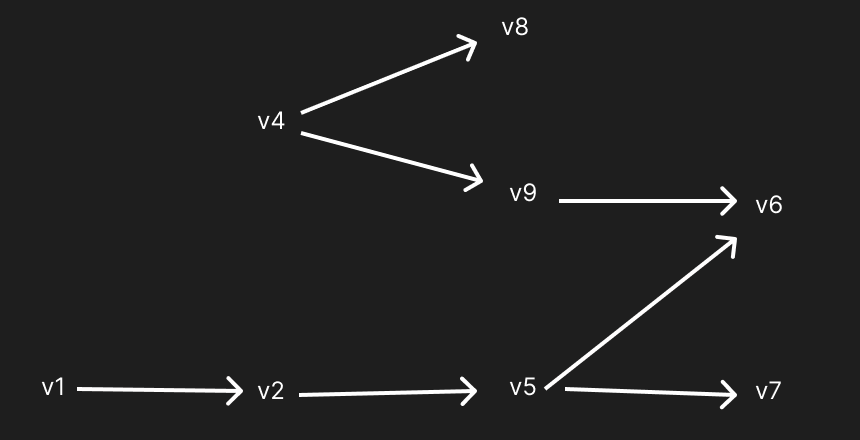
\includegraphics[width=0.7\textwidth]{pics/1.1.png}
    \caption{Изображение ориентированного графа}
    \label{p1}
\end{figure} 

Тогда после выполнении программы результатом будет являться следующая структура, которая
будет записана в файл формата JSON.

\begin{minted}{JSON}
    {
        "graph": 
        {
            "vertex": 
            [
                "v1", "v2", "v3", "v4", "v5", 
                "v6", "v7", "v8", "v9"
            ], 
            "arc": 
            [
                {"from": "v1", "to": "v2", "order": 1}, 
                {"from": "v3", "to": "v4", "order": 1}, 
                {"from": "v2", "to": "v5", "order": 1}, 
                {"from": "v5", "to": "v6", "order": 1}, 
                {"from": "v5", "to": "v7", "order": 1}, 
                {"from": "v4", "to": "v8", "order": 1}, 
                {"from": "v4", "to": "v9", "order": 1}, 
                {"from": "v9", "to": "v6", "order": 2}
            ]
        }
    }
    \end{minted}

\textbf{Пример 2:}

Рассмотрим ориентированный граф, который имеет следующую запись:

\begin{center}
    $(a, b, 1),(c, d, 1),(b, e, 1),(d, e, 1),(e, f, 1)$
\end{center}

На рисунке \ref{p2} показано изображение данного графа.

\begin{figure}[H]
    \centering
    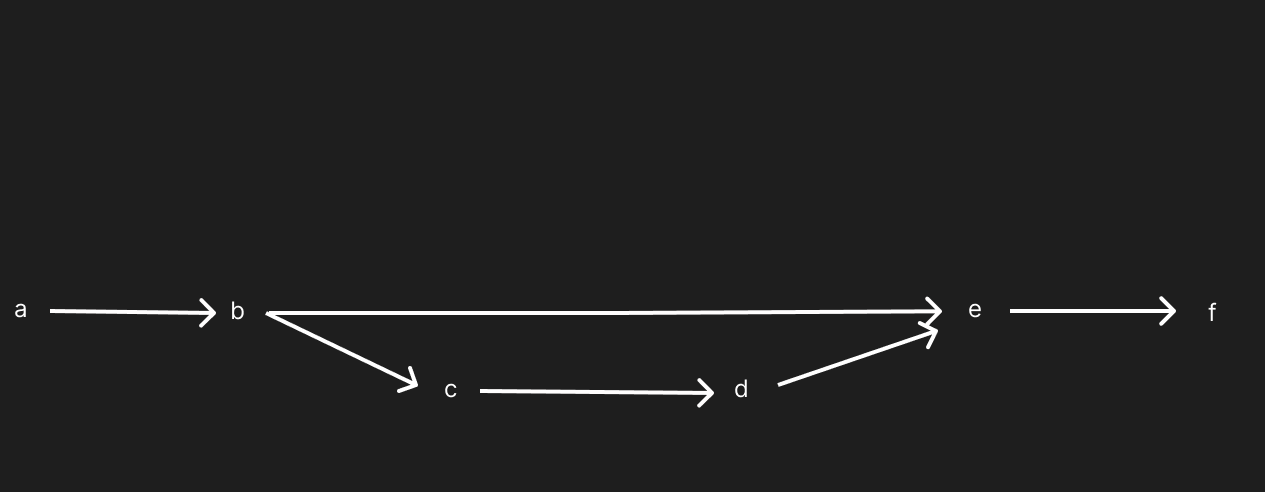
\includegraphics[width=0.7\textwidth]{pics/1.2.png}
    \caption{Изображение ориентированного графа}
    \label{p2}
\end{figure} 

Исходя из рисунка, можно заметить, что такой вариант графа вполне допустим, однако в описании дуг
была допущена ошибка: дуги $(b, e, 1)$ и $(d, e, 1)$ имеют одинаковый порядковый 
номер. В таком случае программа выводит сообщение об ошибке, что в графе некорректно заданы
номера.

\section{Создание функции по графу}

    \subsection{Описание задачи №2}

        \textbf{На входе:} ориентированный граф с именованными вершинами как 
        описано в задании 1.
        
        \textbf{На выходе:} линейное представление функции, реализуемой графом в префиксной скобочной записи:

            \begin{center}
                $A_1(B_1(C_1(\dots), \dots, C_m(\dots)), \dots, B_n(\dots))$
            \end{center}

        \textbf{Способ проверки резульата:}
            \begin{itemize}
                \item[а)] выгрузка в текстовый файл результата преобразования графа в имя функции.
                \item[б)] сообщение о наличии циклов в графе, если они присутствуют.
            \end{itemize}
        
    \subsection{Примеры исполнения программы}


    \textbf{Пример 1:}

    Рассмотрим ориентированный граф, который имеет следующую запись:

    \begin{center}
        $(v1, v2, 1), (v3 , v2, 2), (v2, v4, 1), (v4, v5, 1)$
    \end{center}

    На рисунке \ref{p21} показано изображение данного графа.

    \begin{figure}[H]
        \centering
        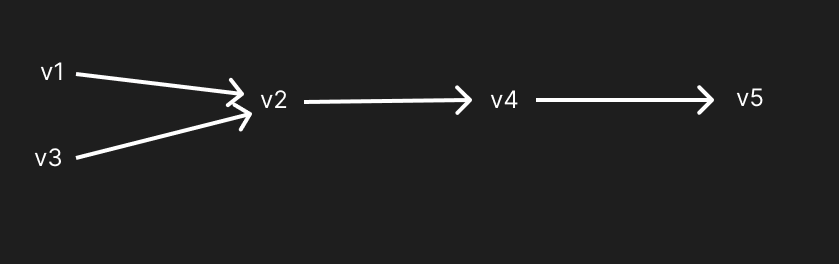
\includegraphics[width=0.7\textwidth]{pics/2.1.png}
        \caption{Изображение ориентированного графа}
        \label{p21}
    \end{figure} 

    В результате работы программы в файл будет сделана следующая запись:

    \begin{center}
        $v5(v4(v2(v1(), v3())))$
    \end{center}


    \textbf{Пример 2:}

    Рассмотрим ориентированный граф, который имеет следующую запись:

    \begin{center}
        $(v1, v2, 1), (v2, v3, 1), (v3, v1, 1)$
    \end{center}

    На рисунке \ref{p22} показано изображение данного графа.

    \begin{figure}[H]
        \centering
        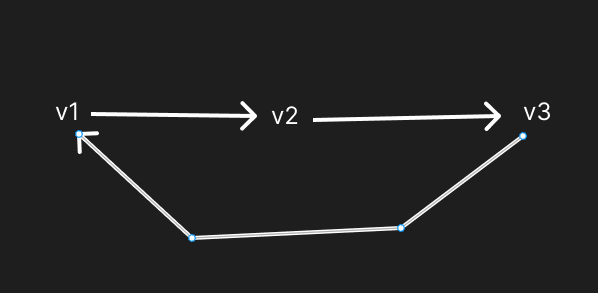
\includegraphics[width=0.7\textwidth]{pics/2.2.png}
        \caption{Изображение ориентированного графа}
        \label{p22}
    \end{figure} 

    Исходя из рисунка, видно, что в данном графе присутствует цикл. Поэтому результатом
    программы будет вывод об ошибке в консоль.


\section{Вычисление значение функции на графе}

    \subsection{Описание задачи №3}

    \textbf{На входе:} 

        \begin{itemize}
            \item[а)] Текстовый файл с описанием графа в виде списка дуг (смотри задание 1).
            \item[б)] Текстовый файл соответствий арифметических операций именам вершин:
            
                \begin{center}
                    $a_1 : 1\text{-я операция}$ \\
                    $a_2 : 2\text{-я операция}$ \\
                    $\dots$ \\
                    $a_n : n\text{-я операция}$, \\
                \end{center}
                где $a_i$ -- имя $i$-й вершины, $i$-я операция -- символ операции, соответствующий вершине $a_i$.
                
                Допустимы следующие символы операций: \\
                $+$ -- cумма значений,\\
                $*$ -- произведение значений,\\
                $exp$ -- экспонирование входного значения,\\
                число -- любая числовая константа.\\		
        \end{itemize}

    \textbf{На выходе:} значение функции, построенной по графу а) и файлу б).

    \textbf{Способ проверки результата:} результат вычисления, выведенный в файл.

    \subsection{Примеры исполнения программы}
    
    \textbf{Пример 1:}

    Рассмотрим ориентированный граф, который имеет следующую запись:

    \begin{center}
        $(v1, v2, 1), (v1, v2, 2), (v2, v6, 1), (v3, v5, 1), (v4, v5, 2), (v6, v7, 1), (v5, v7, 2)$
    \end{center}

    Также имеются соответствия арифметических операций именам вершинам, записанных в файле формата JSON:

    \begin{minted}{JSON}
        {
            "v1" : 1,
            "v2" : "+",
            "v3" : 5,
            "v4" : 12,
            "v5" : "*",
            "v6" : "exp",
            "v7" : "+"
        }
    \end{minted}
    
    На рисунке \ref{p31} показано изображение данного графа.

    \begin{figure}[H]
        \centering
        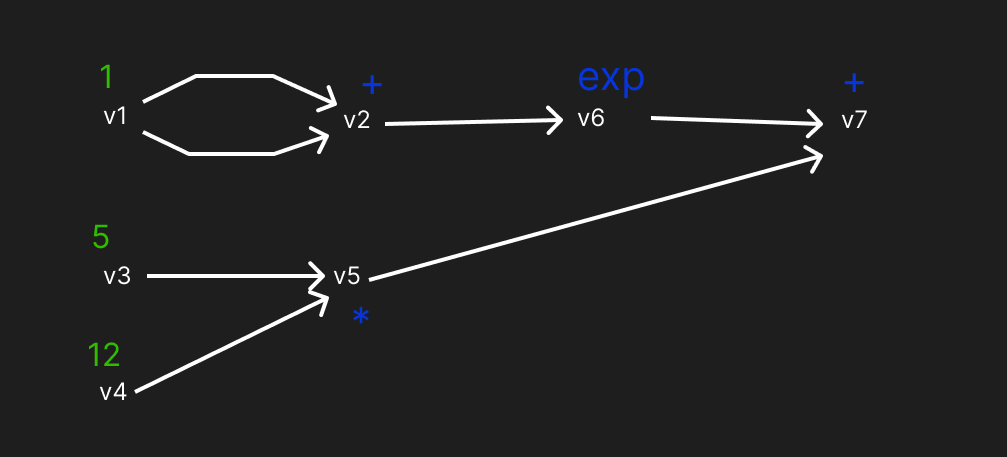
\includegraphics[width=0.7\textwidth]{pics/3.1.png}
        \caption{Изображение ориентированного графа}
        \label{p31}
    \end{figure} 

    После всех проверок входных данных на корректность, программа 
    представляет ориентированный граф в следующем виде:
    
    \begin{center}
        $v7(v6(v2(v1(), v1())), v5(v3(), v4()))$
    \end{center}

    Подставив в соответствие именам вершин арифметические операции получается следующая запись:

    \begin{center}
        $+(exp(+(1, 1)), *(5, 12))$
    \end{center}

    Таким образом программе необходимо вычислить выражение, представленное в префиксной записи.
    В итоге программа записывает в текстовый файл результат данного выражения: 67.38905609893065.

    \textbf{Пример 2:}

    Теперь рассмотрим ориентированный граф, который имеет достаточную простую запись:

    \begin{center}
        $(v1, v3, 1), (v2, v3, 2)$
    \end{center}

    Также имеются следующие соответствия:

    \begin{minted}{JSON}
        {
            "v1" : 1,
            "v2" : "+",
            "v3" : 5
        }
    \end{minted}
    
    На рисунке \ref{p32} показано изображение данного графа.

    \begin{figure}[H]
        \centering
        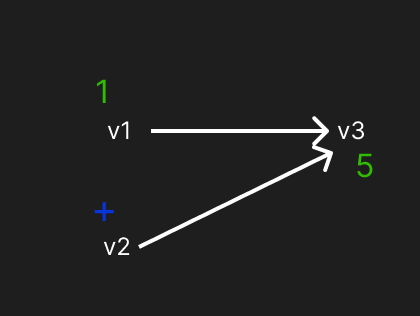
\includegraphics[width=0.7\textwidth]{pics/3.2.png}
        \caption{Изображение ориентированного графа}
        \label{p32}
    \end{figure} 

    Исходя из рисунка и текущих соответствий, можно заметить, что в данном случае невозможно
    будет вычислить результат. Поэтому программа выдает в качестве ответа в консоль сообщение
    об ошибке.

\section{Построение многослойной нейронной сети}

\subsection{Описание задачи №4}

    \textbf{На входе:} 

    \begin{itemize}
        \item[а)] Текстовый файл с набором матриц весов межнейронных связей:
        \begin{center}
            $M_1 : [a_{11}^1, a_{12}^1, \dots, a_{1n_1}^1], \dots, [a_{m_11}^1, a_{m_12}^1, \dots ,a_{m_1n_1}^1]$ \\
            $M_2 : [a_{11}^2, a_{12}^2, \dots, a_{1n_2}^2], \dots, [a_{m_21}^2, a_{m_22}^2, \dots ,a_{m_2n_2}^2]$\\
            $\dots$\\
            $M_p : [a_{11}^p, a_{12}^p, \dots, a_{1n_p}^p], \dots, [a_{m_p1}^p, a_{m_p2}^p, \dots,a_{m_pn_p}^p]$ \\                  
        \end{center}
        \item[б)] Текстовый файл с входным вектором в формате:
        
        \begin{center}
            $x_1, x_2, \dots, x_k$.
        \end{center}
    \end{itemize}

    \textbf{На выходе:}
        \begin{itemize}
            \item[а)] Сериализованная многослойная нейронная сеть (в формате XML или JSON) с полносвязной межслойной структурой. 
            Файл с выходным вектором -- результатом вычислений НС в формате: 
            \begin{center}
                $y_1, y_2, \dots, y_k.$                
            \end{center}
            \item[б)] Сообщение об ошибке, если в формате входного вектора или файла описания НС допущена 
            ошибка.
        \end{itemize}
        

\subsection{Примеры исполнения программы}


\section{Реализация метода обратного распространения ошибки для многослойной НС}

    \subsection{Описание задачи №5}

        \textbf{На входе:}
        
            \begin{itemize}
                \item[а)] Текстовый файл с описанием НС (формат см. в задании 4).
                \item[б)] Текстовый файл с обучающей выборкой:
                
                    \begin{center}
                        $[x_{11}, x_{12}, \dots, x_{1n}] \rightarrow [y_{11}, y_{12}, \dots, y_{1m}]$ \\
                        $\dots$\\
                        $[x_{k1}, x_{k2}, \dots, x_{kn}] \rightarrow [y_{k1}, y_{k2}, \dots, y_{km}]$ \\
                    \end{center}
                    Формат описания входного вектора x и выходного вектора y соответствует формату из задания 4. 
                \item[в)] Число итераций обучения (в строке параметров).

            \end{itemize}

        \textbf{На выходе:} Текстовый файл с историей $N$ итераций обучения методом обратного распространения ошибки:
            \begin{center}
                $1 : \text{1-я ошибка}$ \\
                $2 : \text{2-я ошибка}$ \\
                    $\dots$\\
                $N : \text{N-я ошибка}$ \\

            \end{center}
\end{document}